\section{Results}
\label{sec:results}

This section shows the results of our model performance and the user evaluation of our service implementation.

\subsection{Machine Learning}
\label{sec:learning}

We used the training data of 475 projects on three commonly used machine learning algorithms.
The projects varied in size and the algorithms we tested are: Logistic Regression, Naive Bayes and Random Forest.
We ran the three algorithms against each project with a 10-fold cross-validation.
The models were trained with 90\% of the training data, the remaining 10\% was used as test data.

In table~\ref{tab:alg-compare} it can be seen how the three algorithms performed.
Both LR and NB perform well on recall, but have a very low precision which makes it unusable for our application.
The RF algorithm performs less on recall, but achieves a higher precision, which is more important in our case.
High precision means that the algorithm returned substantially more relevant results than irrelevant.
It seems that RF is the best at identifying the important pull requests.

\begin{table}
  \begin{tabular}{lrrrrc}
    \hline
    \textbf{Algorithm} & \textbf{5\%} & \textbf{Mean} & \textbf{Median} & \textbf{95\%} & \textbf{Histogram} \\
    \hline

    \bf{Logistic Regression}\\
    Area Under Curve & 0.71 & 0.81 & 0.81 & 0.91 & \includegraphics[scale = 0.1, clip = true, trim= 50px 60px 50px 60px]{../figs/hist-results/hist-LRauc.pdf} \\
    Accuracy & 0.52 & 0.62 & 0.62 & 0.72 & \includegraphics[scale = 0.1, clip = true, trim= 50px 60px 50px 60px]{../figs/hist-results/hist-LRacc.pdf} \\
    Precision & 0.06 & 0.36 & 0.30 & 0.88 & \includegraphics[scale = 0.1, clip = true, trim= 50px 60px 50px 60px]{../figs/hist-results/hist-LRprec.pdf} \\
    Recall & 0.66 & 0.83 & 0.84 & 0.95 & \includegraphics[scale = 0.1, clip = true, trim= 50px 60px 50px 60px]{../figs/hist-results/hist-LRrec.pdf} \\
    F1 & 0.12 & 0.45 & 0.44 & 0.77 & \includegraphics[scale = 0.1, clip = true, trim= 50px 60px 50px 60px]{../figs/hist-results/hist-LRf1.pdf} \\

    \bf{Naive Bayes}\\
    Area Under Curve & 0.65 & 0.75 & 0.75 & 0.86 & \includegraphics[scale = 0.1, clip = true, trim= 50px 60px 50px 60px]{../figs/hist-results/hist-NBauc.pdf} \\
    Accuracy & 0.52 & 0.60 & 0.60 & 0.69 & \includegraphics[scale = 0.1, clip = true, trim= 50px 60px 50px 60px]{../figs/hist-results/hist-NBacc.pdf} \\
    Precision & 0.06 & 0.34 & 0.28 & 0.82 & \includegraphics[scale = 0.1, clip = true, trim= 50px 60px 50px 60px]{../figs/hist-results/hist-NBprec.pdf} \\
    Recall & 0.63 & 0.79 & 0.80 & 0.94 & \includegraphics[scale = 0.1, clip = true, trim= 50px 60px 50px 60px]{../figs/hist-results/hist-NBrec.pdf} \\
    F1 & 0.11 & 0.42 & 0.41 & 0.73 & \includegraphics[scale = 0.1, clip = true, trim= 50px 60px 50px 60px]{../figs/hist-results/hist-NBf1.pdf} \\

    \bf{Random Forest}\\
    Area Under Curve & 0.81 & 0.89 & 0.89 & 0.95 & \includegraphics[scale = 0.1, clip = true, trim= 50px 60px 50px 60px]{../figs/hist-results/hist-RFauc.pdf} \\
    Accuracy & 0.73 & 0.86 & 0.87 & 0.96 & \includegraphics[scale = 0.1, clip = true, trim= 50px 60px 50px 60px]{../figs/hist-results/hist-RFacc.pdf} \\
    Precision & 0.37 & 0.66 & 0.69 & 0.90 & \includegraphics[scale = 0.1, clip = true, trim= 50px 60px 50px 60px]{../figs/hist-results/hist-RFprec.pdf} \\
    Recall & 0.36 & 0.62 & 0.63 & 0.84 & \includegraphics[scale = 0.1, clip = true, trim= 50px 60px 50px 60px]{../figs/hist-results/hist-RFrec.pdf} \\
    F1 & 0.38 & 0.63 & 0.63 & 0.87 & \includegraphics[scale = 0.1, clip = true, trim= 50px 60px 50px 60px]{../figs/hist-results/hist-RFf1.pdf} \\
    \hline
  \end{tabular}
  \caption[Comparision of algorithms]{Comparision of algorithms. Scores and distributions of algorithm performance.}
  \label{tab:alg-compare}
\end{table}

The results in table~\ref{tab:alg-compare} led us believe that there was room for improvement.
Since the important snapshot data vs. unimportant data is very imbalanced, we decided to tune the balance.
However, balancing the data turned out to make things worse.

It is interesting to see that the age is a very dominant factor when we look at the feature importance in figure~\ref{fig:feature-importance}.
This is probably the case because it is very likely that new pull requests receive comments within the first few days.
Since the age feature is so dominant it could impact the model in a bad way.
When we turned this particular feature off, the results were worse instead.
So it seems the age has a positive effect on the prediction.

\begin{figure}
  \centering
  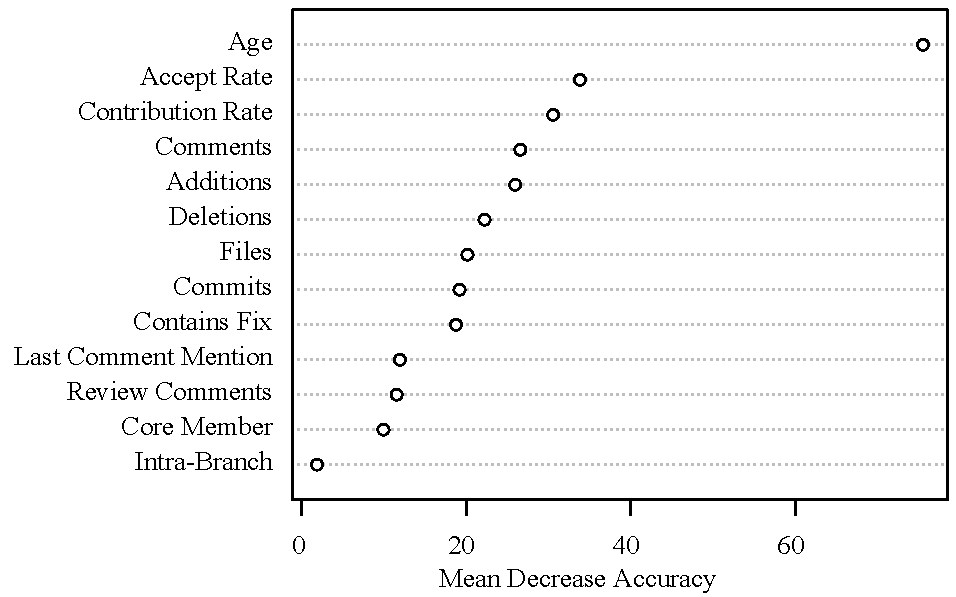
\includegraphics[width=0.45\textwidth]{../figs/mean-decrease-accuracy.pdf}
  \caption[Plot of feature importance]
   {Plot of feature importance of the aggregated projects. The age of the pull request is the dominant factor.}
  \label{fig:feature-importance}
\end{figure}

Despite the fact that it should be possible to further improve the prediction model and because this is only a preliminary study to prioritizing pull requests, we decided to go forward with the current model.

\subsection{Evaluation}
\label{sec:evaluation}

\erik{Discuss questionnaire here.}
